\documentclass[12pt]{article}
\usepackage{graphicx}
\usepackage{hyperref}
\usepackage[top=2.75in, left=1in, right=1in, bottom=0.25in]{geometry}
\usepackage[utf8]{inputenc}
\usepackage[english]{babel}
\usepackage{fancyhdr}
\usepackage[utf8]{inputenc}
\usepackage{listings}
\usepackage{color}
\usepackage[final]{pdfpages}
\usepackage{multirow}
\usepackage{array}
\usepackage{caption}
\usepackage{subcaption}


\definecolor{codegreen}{rgb}{0,0.6,0}
\definecolor{codegray}{rgb}{0.5,0.5,0.5}
\definecolor{codepurple}{rgb}{0.58,0,0.82}
\definecolor{backcolour}{rgb}{0.95,0.95,0.92} 
\lstdefinestyle{mystyle}{
    backgroundcolor=\color{backcolour},   
    commentstyle=\color{codegreen},
    keywordstyle=\color{magenta},
    numberstyle=\tiny\color{codegray},
    stringstyle=\color{codepurple},
    basicstyle=\footnotesize,
    breakatwhitespace=false,         
    breaklines=true,                 
    captionpos=b,                    
    keepspaces=true,                 
    numbers=left,                    
    numbersep=5pt,                  
    showspaces=false,                
    showstringspaces=false,
    showtabs=false,                  
    tabsize=2
} 
\lstset{style=mystyle}

\setlength{\parindent}{4em}
\setlength{\parskip}{1em}
\pagestyle{fancy}
\fancyhf{}
\rhead{Assignment 6}
\lhead{Huan Huang}
\renewcommand{\headrulewidth}{0.4pt}
\renewcommand{\footrulewidth}{0.4pt}
\rfoot{Page \thepage}


\begin{document}
\begin{titlepage}
	\begin{center}
	\Huge{Web Science cs532-s16}\\
	[0.25in]
	\textsc{\Large Assignment 6 Report}\\
	\textsc{\normalsize Dr. Michael L. Nelson}\\
	[4.25in]
	\textsc{\normalsize By: Huan Huang}\\
	\large 03/17/2016\\
	
	
	\end{center}
\end{titlepage}
\newpage

\newgeometry{margin=1in}

\section*{Problem 1}

Use D3 to visualize your Twitter followers.  Use my twitter account
if you do not have more than 50 followers.  For example,
@hvdsomp follows me, as does @mart1nkle1n.  They also follow each
other, so they would both have links to me and links to each other.

\noindent
To see if two users follow each other, see:
\begin{verbatim}
https://dev.twitter.com/rest/reference/get/friendships/show
\end{verbatim}

Attractiveness of the graph counts!  Nodes should be labeled (avatar
images are even better), and edge types (follows, following) should
be marked.

\noindent
Note: for getting GitHub to serve HTML (and other media types), see:
\begin{verbatim}
http://stackoverflow.com/questions/6551446/can-i-run-html-files-directly-from-github-instead-of-just-viewing-their-source
\end{verbatim}

\noindent
Be sure to include the URI(s) for your D3 graph in your report. 

\subsection*{Answer}
To solve this problem, I first dug up my old program from assignment 4 and made some modification to get the screen names of the followers. Also, to make this problem easier, I used one of Mr. Nelson's follower ``jcdl2012" as the source user. He has 70 followers which is much better than Mr. Nelson's 492 followers. 

\lstinputlisting[language=python]{mainFollowers.py}

\begin{figure}[h]
\centering
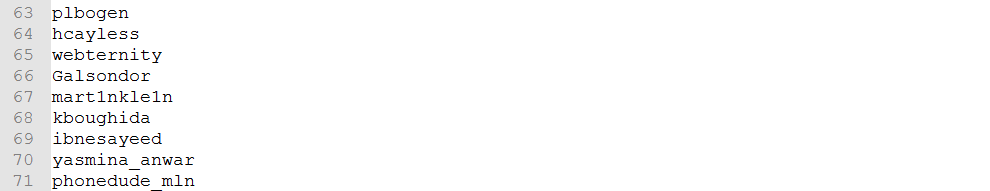
\includegraphics[width=6.5in]{mainfollowers.png}
\caption{Sample of the data file mainfollowers.txt}
\end{figure}

Next, using these screen names, I need to get the relation between each one of them.

\lstinputlisting[language=python]{followFollow.py}

\noindent
Relationship types:\\
0 means A and B are not following eachother\\
1 means A is following B\\
2 means B is following A\\
3 means A and B are following eachother

\begin{figure}[h]
\centering
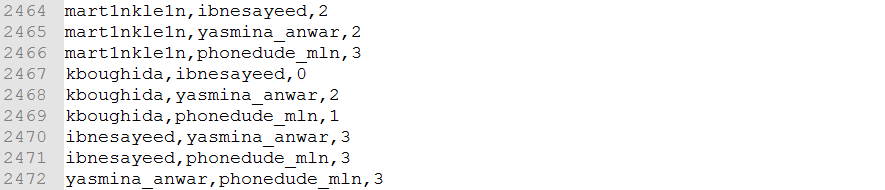
\includegraphics[width=6.5in]{relations.png}
\caption{Sample of the data file relations.txt}
\end{figure}
\newpage

Now, I need convert the data into json file for it to be used in the graph.

\begin{figure}[h]
\centering
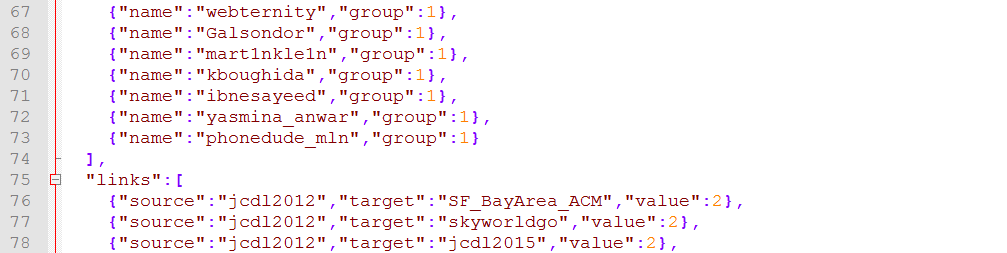
\includegraphics[width=6.5in]{sourceData.png}
\caption{Sample of the data file sourceData.txt}
\end{figure}

Lastly, write the html file to plot the graph with D3.

\lstinputlisting[language=html]{graph.html}

\begin{figure}[h]
\centering
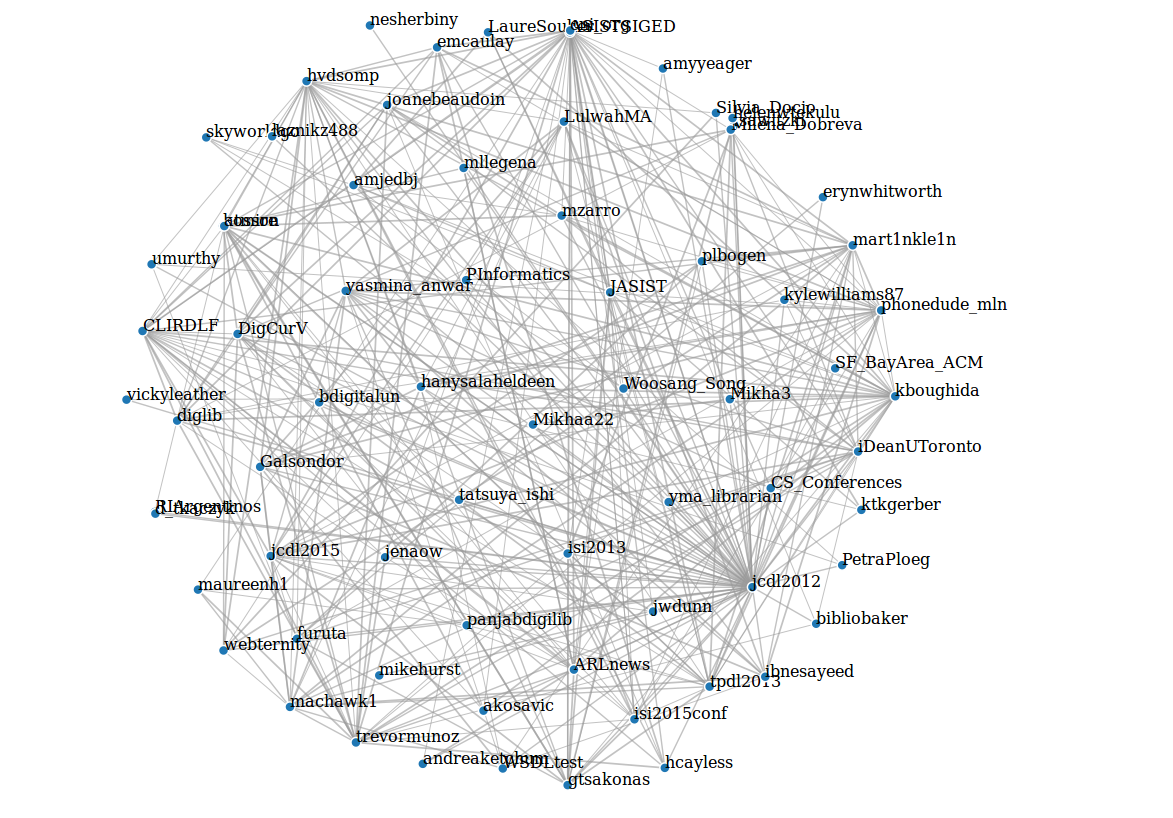
\includegraphics[width=6.5in]{graph.png}
\caption{Graph of the relationship between jcdl2012 and its followers}
\end{figure}

\section*{Problem 2}
Gender homophily in your Twitter graph (5 points)

Take the Twitter graph you generated in question \#1 and test for
male-female homophily.  For the purposes of this question you can
consider the graph as undirected (i.e., no distinction between
``follows" and ``following").  Use the twitter name (not ``screen
name"; for example ``Michael L. Nelson" and not ``@phonedude\_mln")
and programatically determine if the user is male or female.  Some
sites that might be useful:

\begin{verbatim}
https://genderize.io/
https://pypi.python.org/pypi/gender-detector/0.0.4
\end{verbatim}


Create a table of Twitter users and their likely gender.  List any 
accounts that can't be determined and remove them from the graph.


Perform the homophily test as described in slides 11-15, Week 7. Does your Twitter graph exhibit gender homophily?


\subsection*{Answer}


\end{document}